\section{Simulation Results and Discussion}

{\centering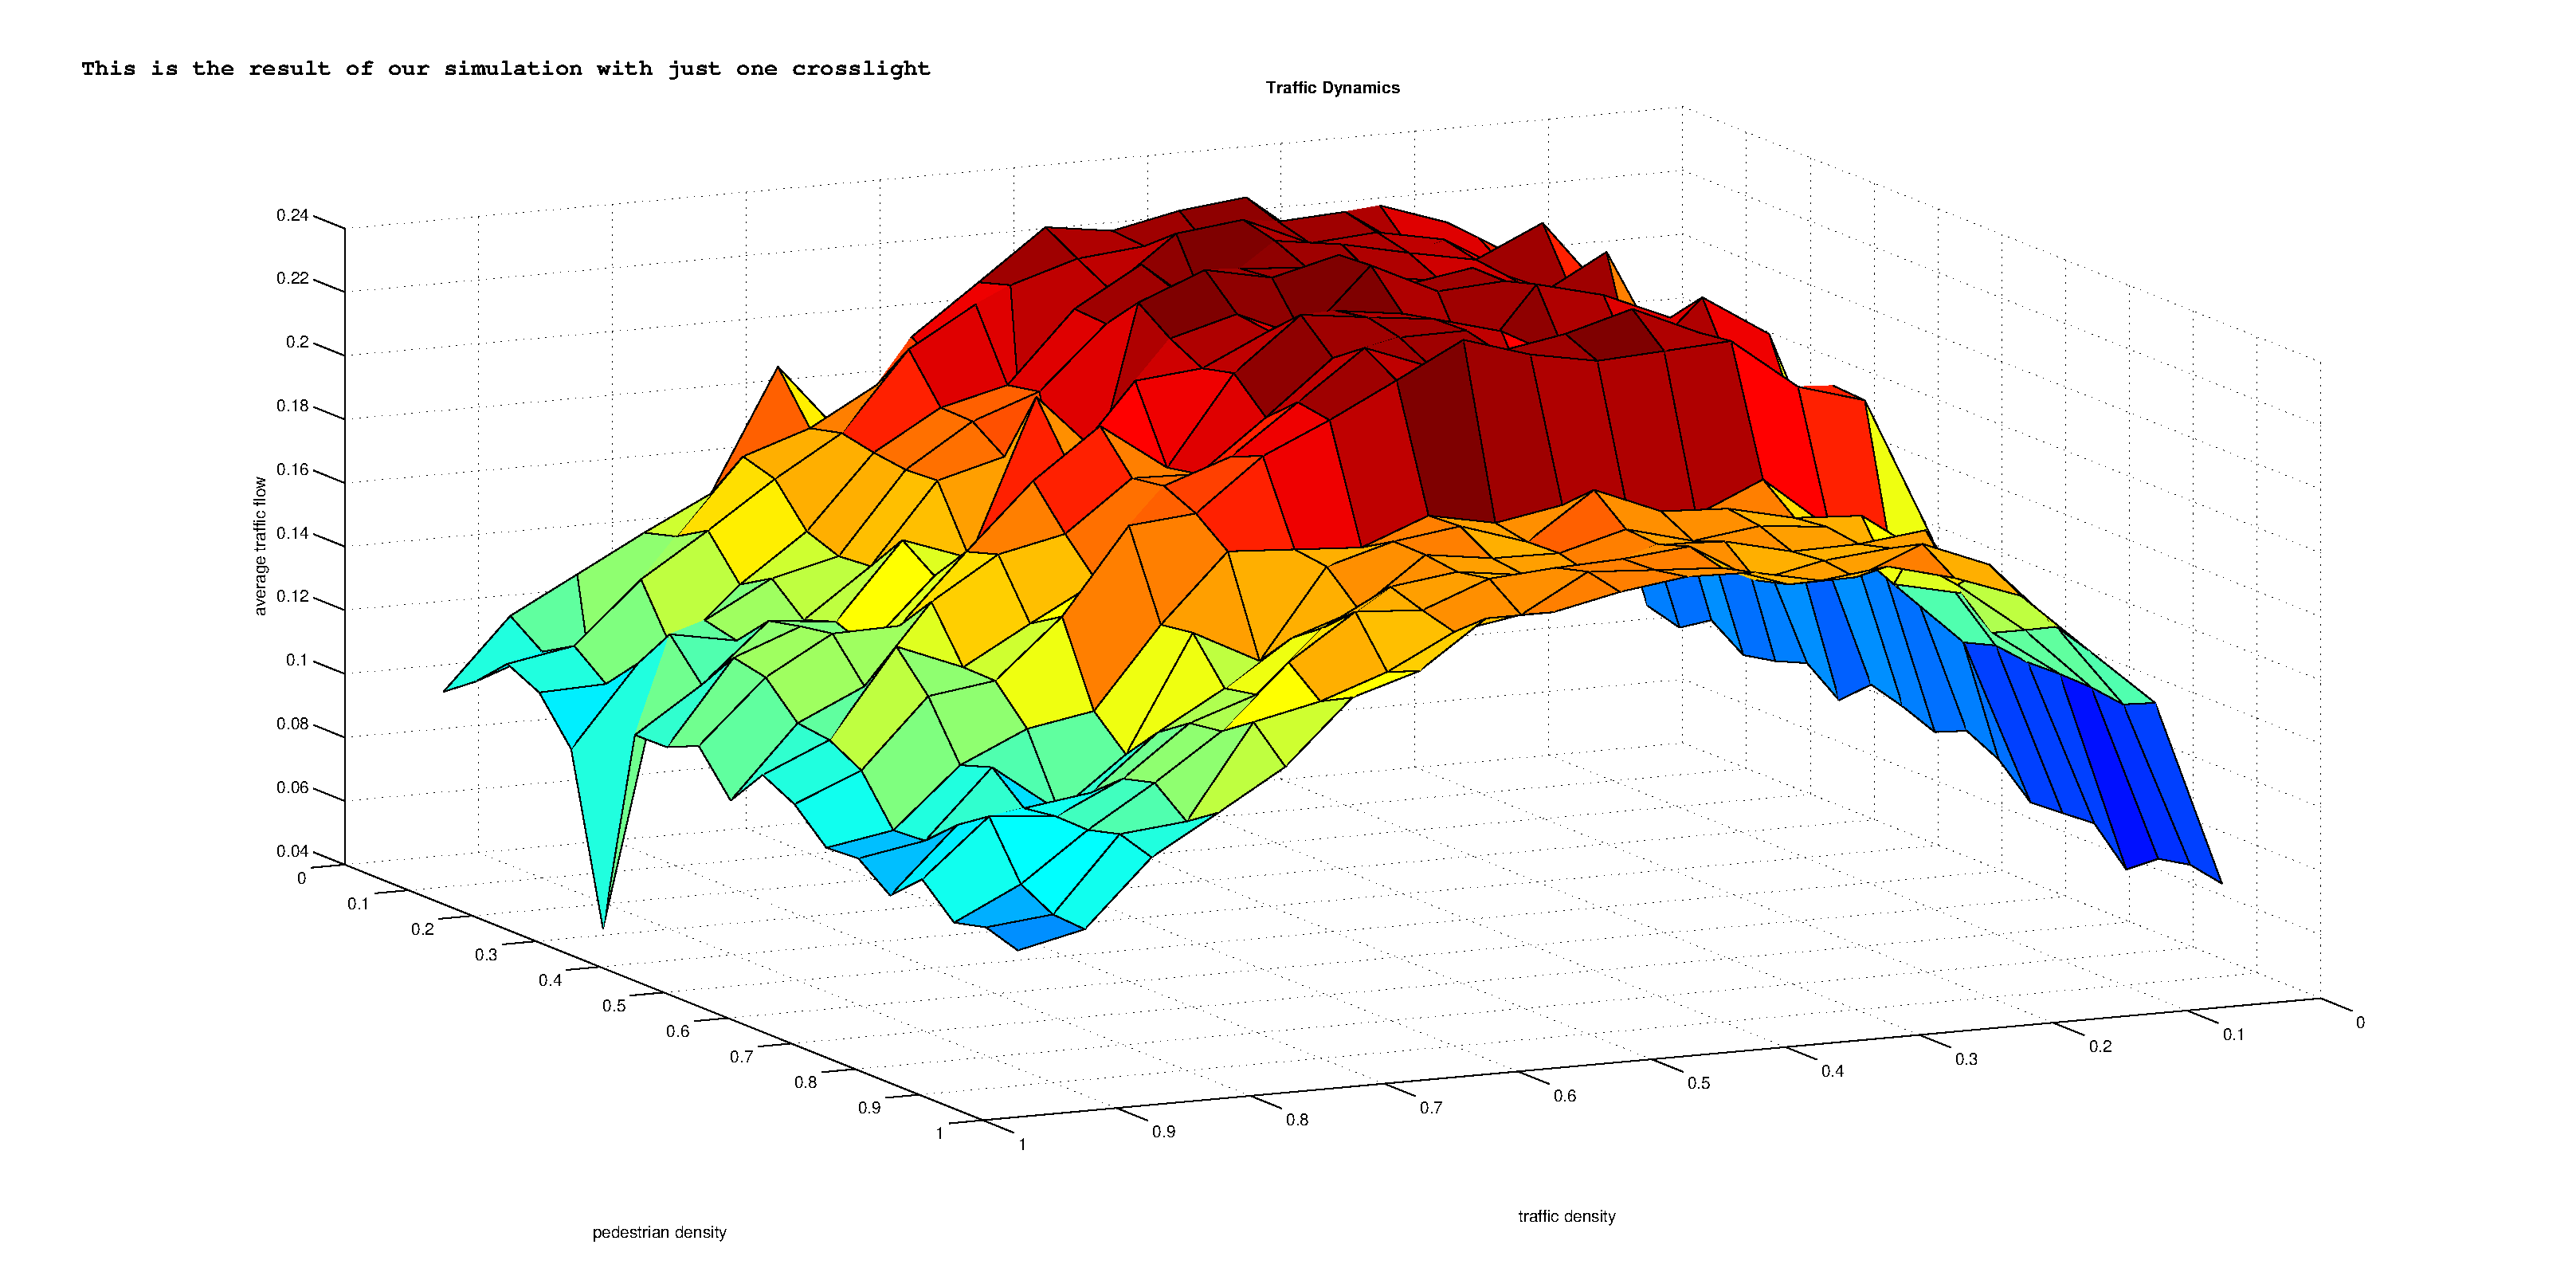
\includegraphics[width=15cm]{images/1-1-trafficlight.eps}

In this plot of one crosslight, one can clearly see the linear increase of traffic flow with increasing car density till ~0.25 after that it is more or less constant till it drops linearly at car densities higher than 0.6. 
One can also see that it does depend only weakly on the pedestrian density, but for high pedestrian densities above ~0.8 we see a small drop. (caused by a different traffic light mode)

{\centering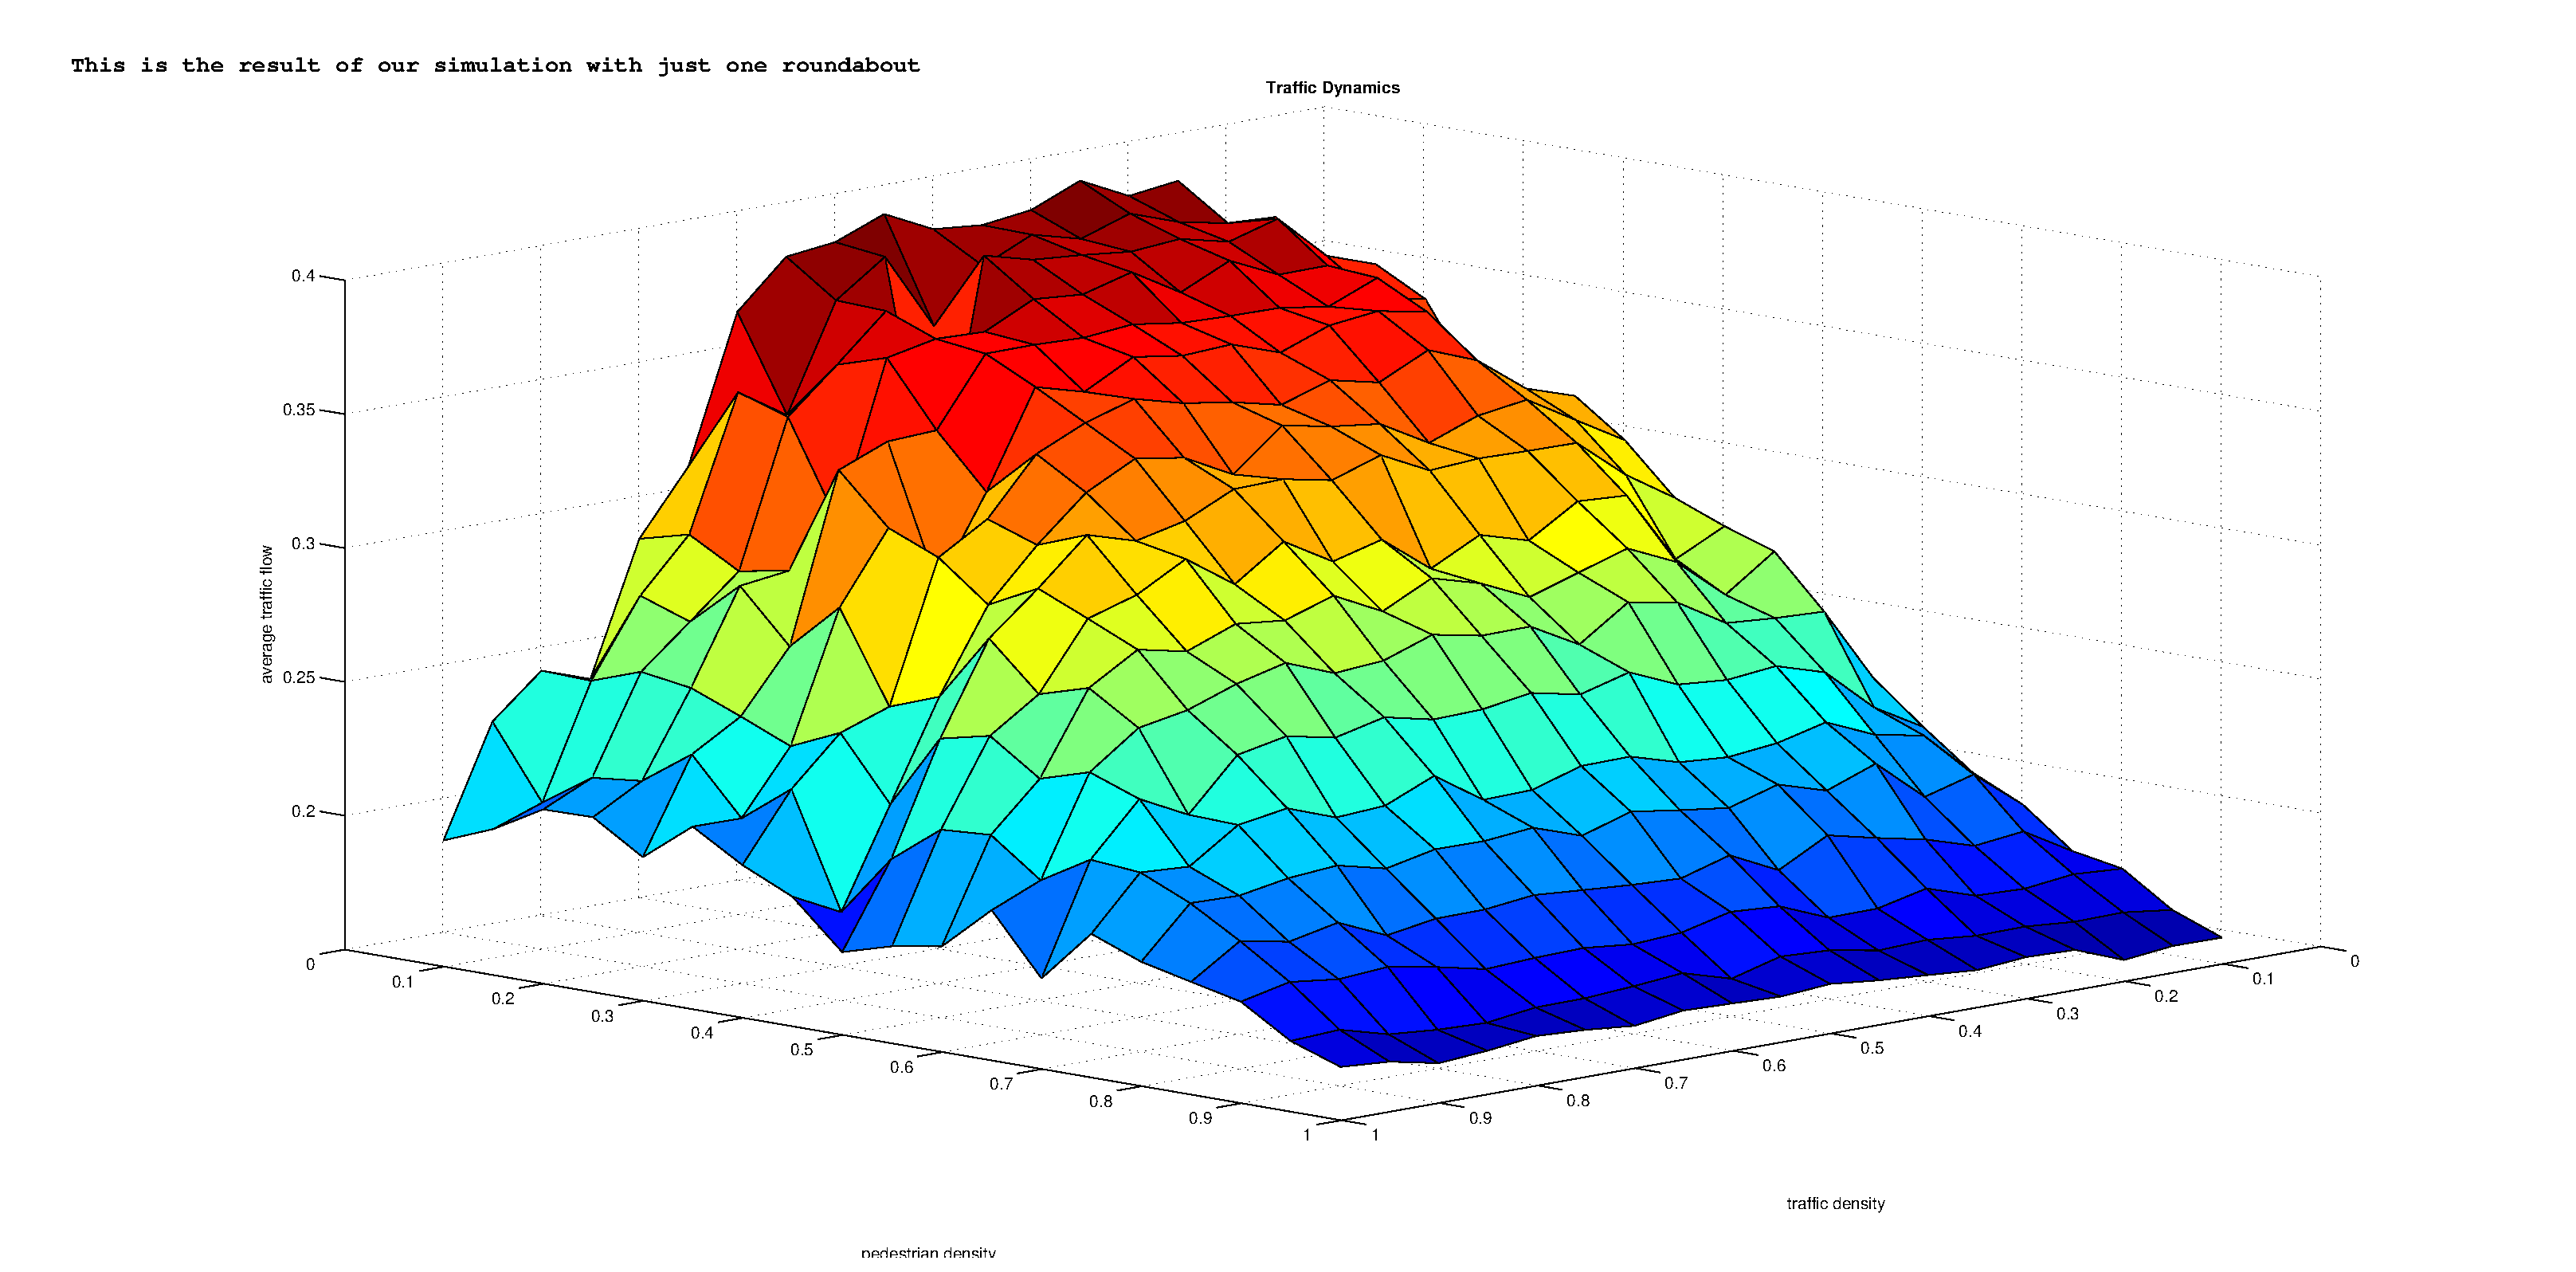
\includegraphics[width=15cm]{images/1-1-roundabout.eps}

In this plot of one roundabout the linear decrease in flow with increasing pedestrian density is clearly visible. And for a const. pedestrian density one sees also the expected result, 
which is a linear increase, then for some time a const flow and ending with a linear decrease for increasing car densities. Compared to the flow of one trafficlight one can see that a roundabout is much more efficient (almost twice the flow) for low pedestrian densities
and less efficient for low densities.

{\centering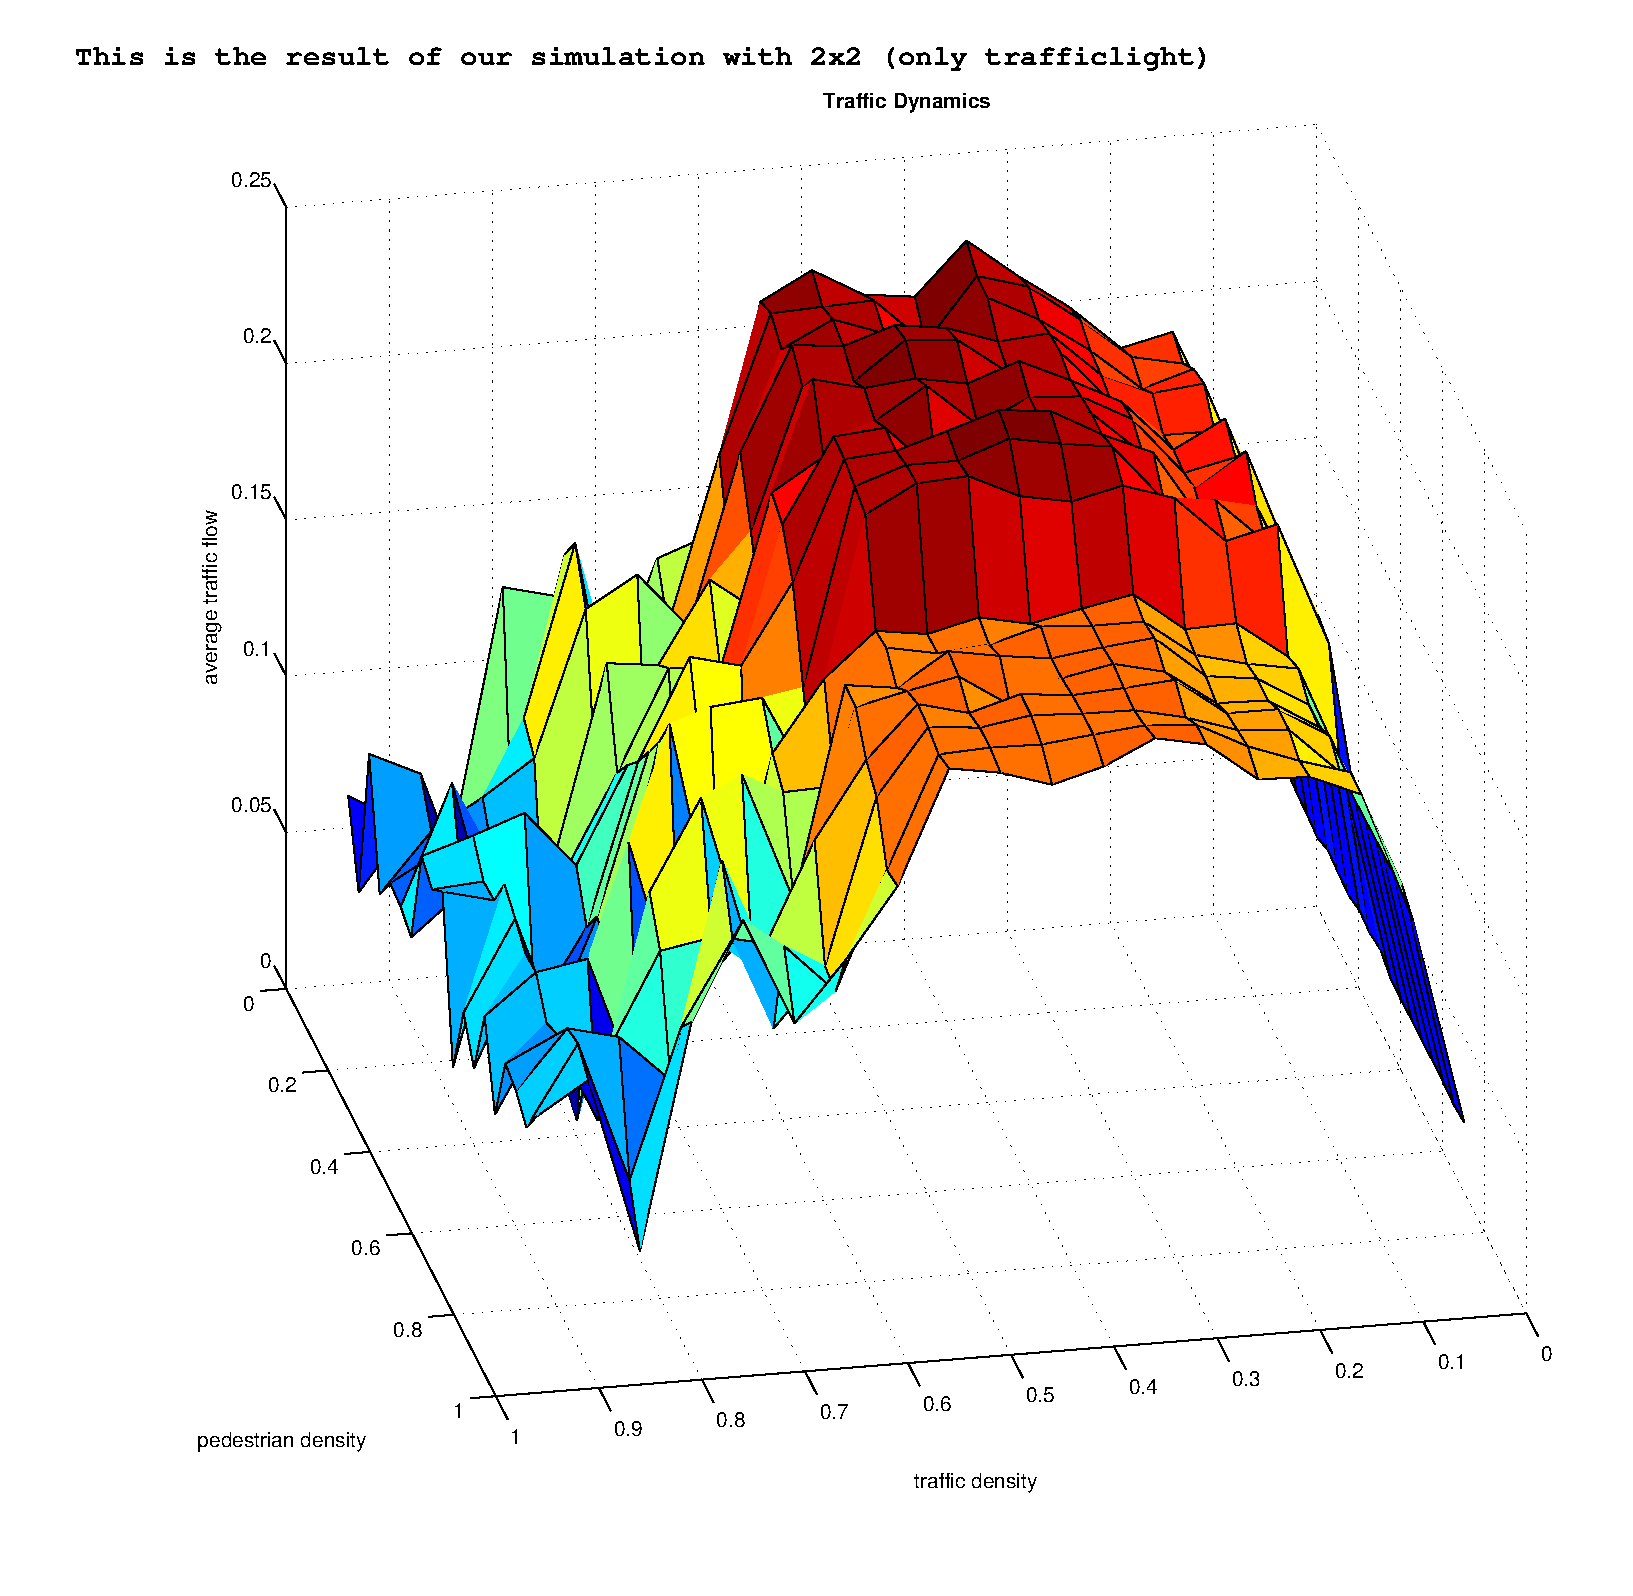
\includegraphics[width=15cm]{images/2-2-trafficlight.eps}

This result does not differ much from the result with just one trafficlight, but one can see that the linear in-/decrease has a higher slope.


{\centering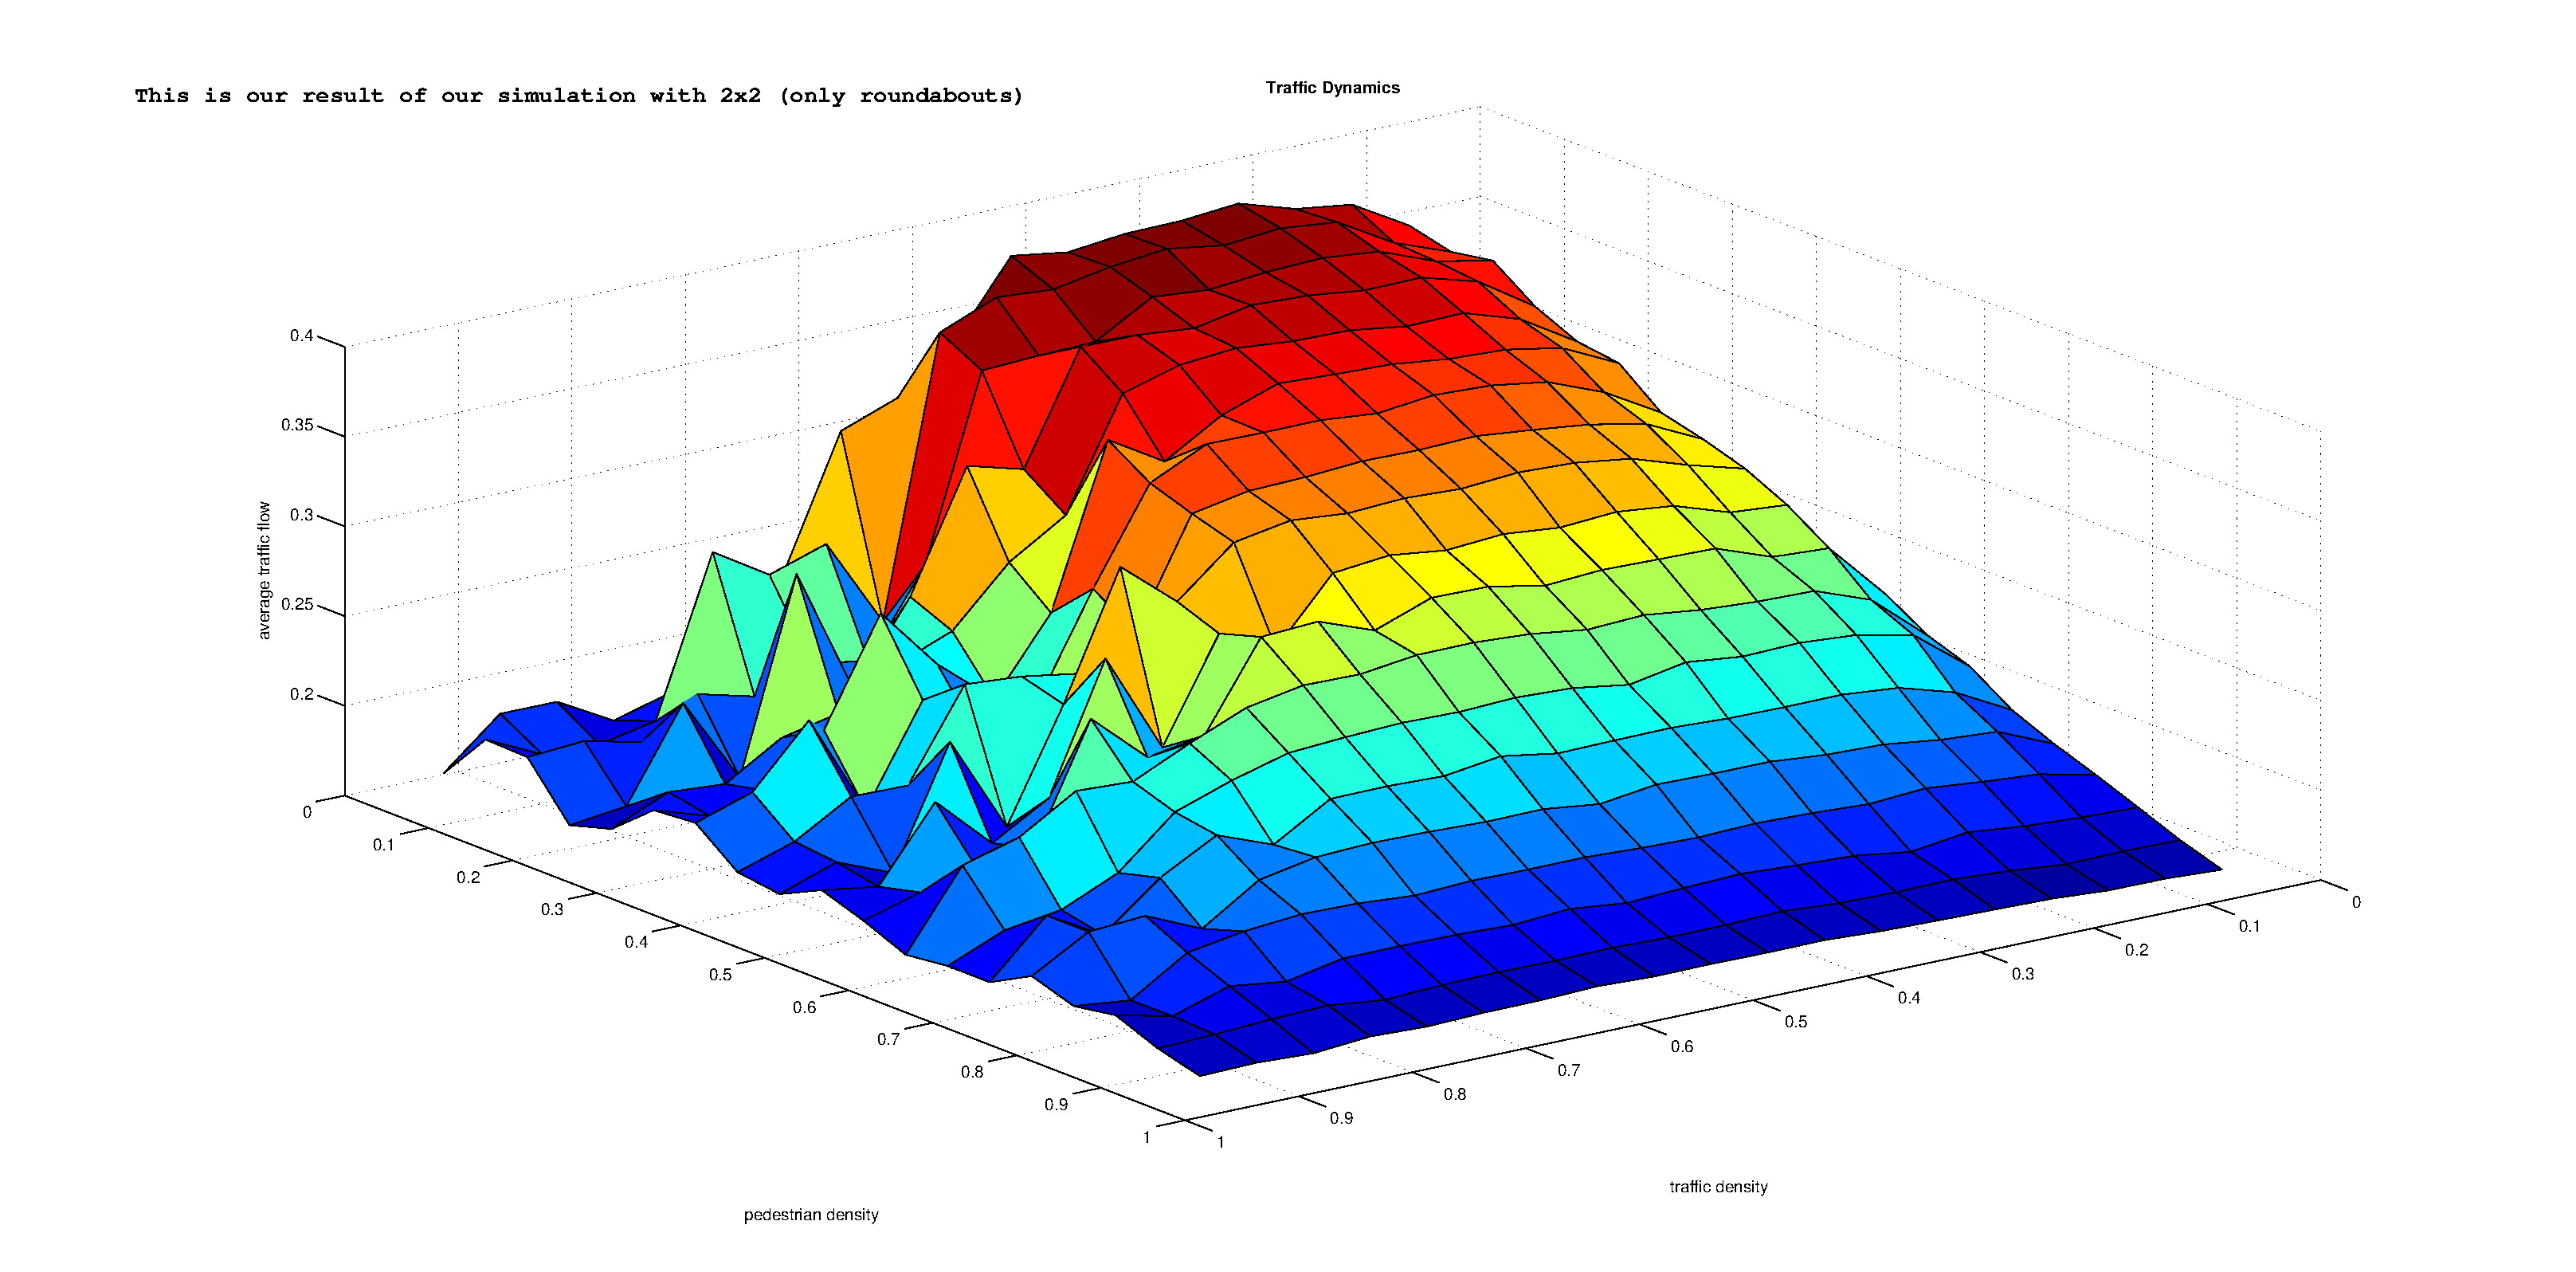
\includegraphics[width=15cm]{images/2-2-roundabout.eps}

This result does not differ much from the single roundabout either, but here the slope of the linear decrease with increasing pedestrian densities is smaller.

{\centering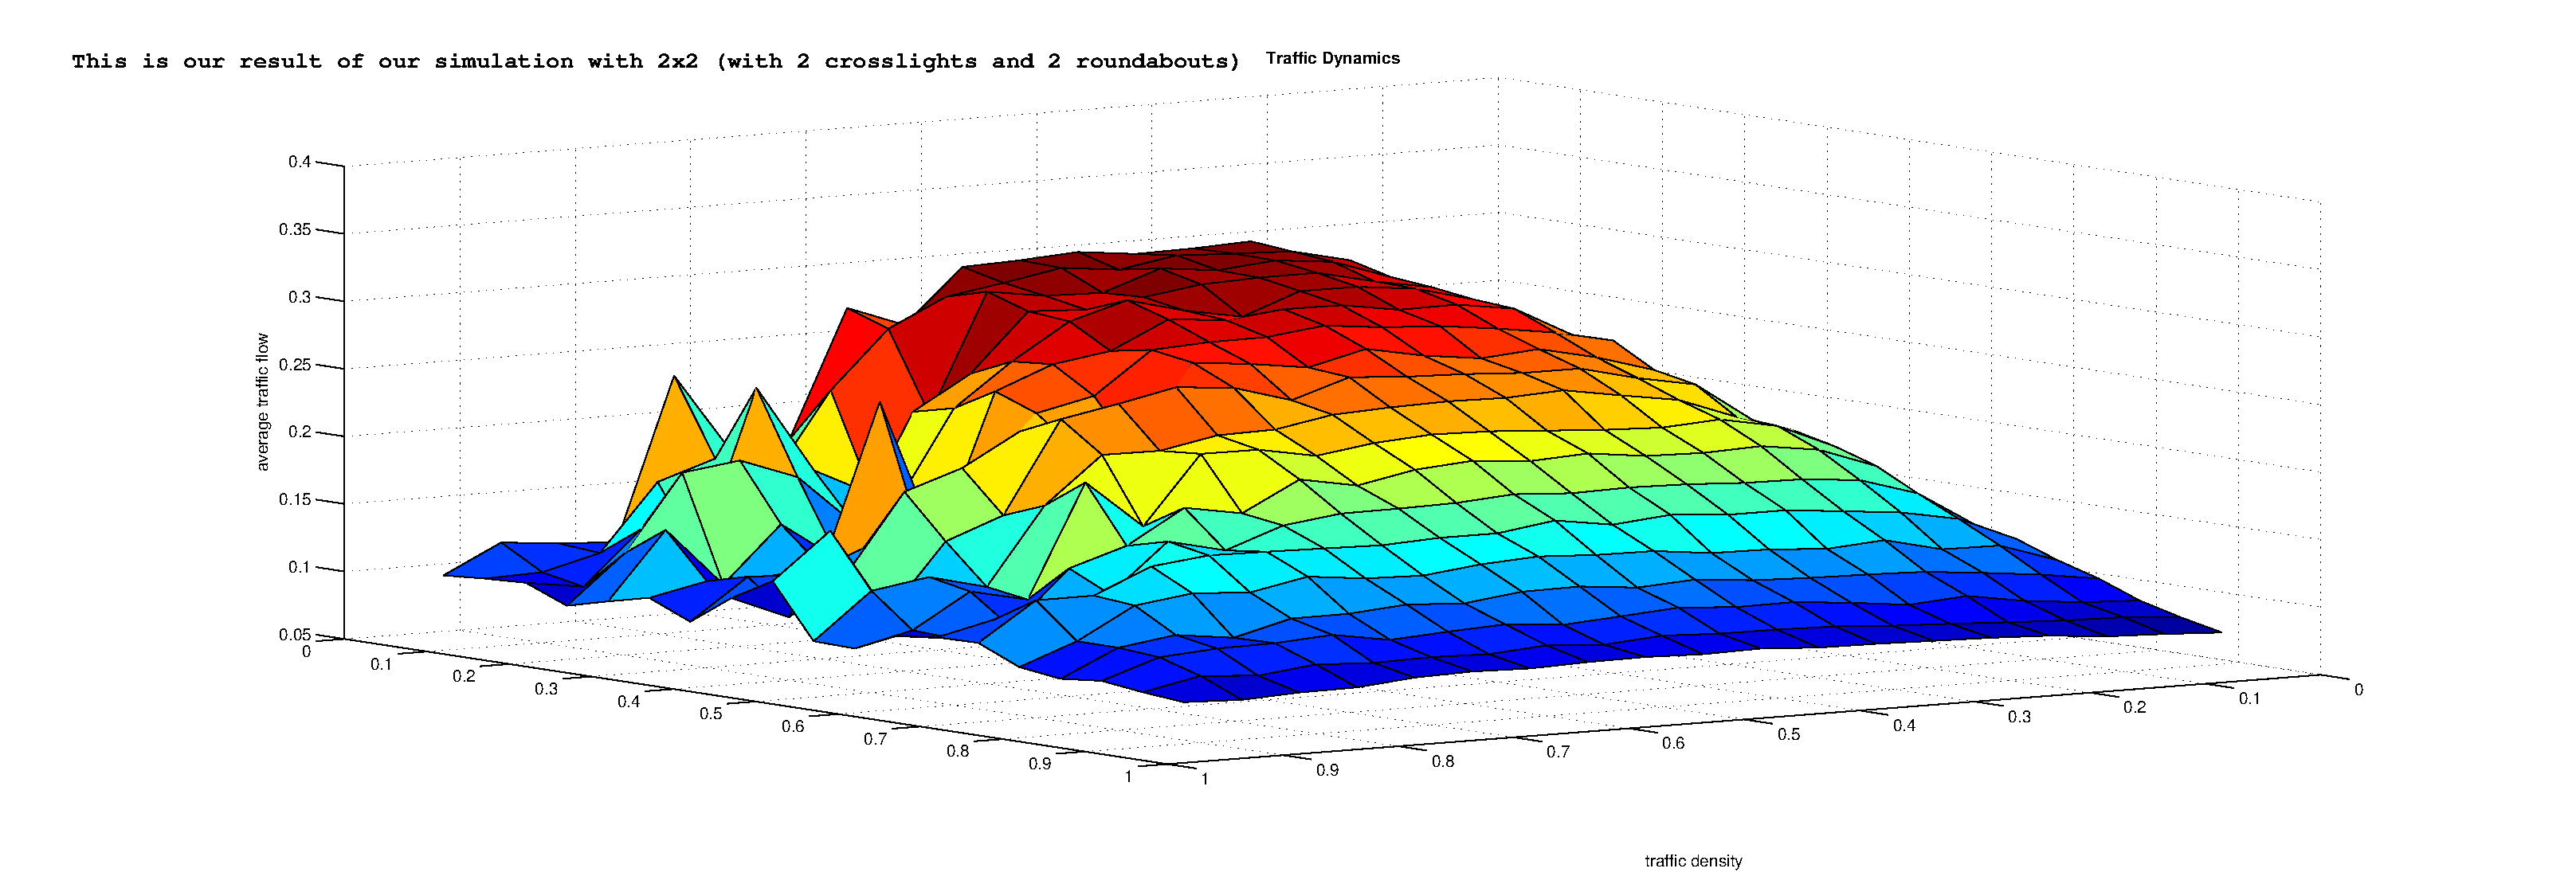
\includegraphics[width=15cm]{images/2-2-mix.eps}

In the combination case of both methods, the characteristic looks dominated by the roundabout (i.e. it does not look much different to the graph above) but here the flow rates are lower. With higher car dnsities random processes are getting more important
and thus the graph does not look so smooth anymore.

{\centering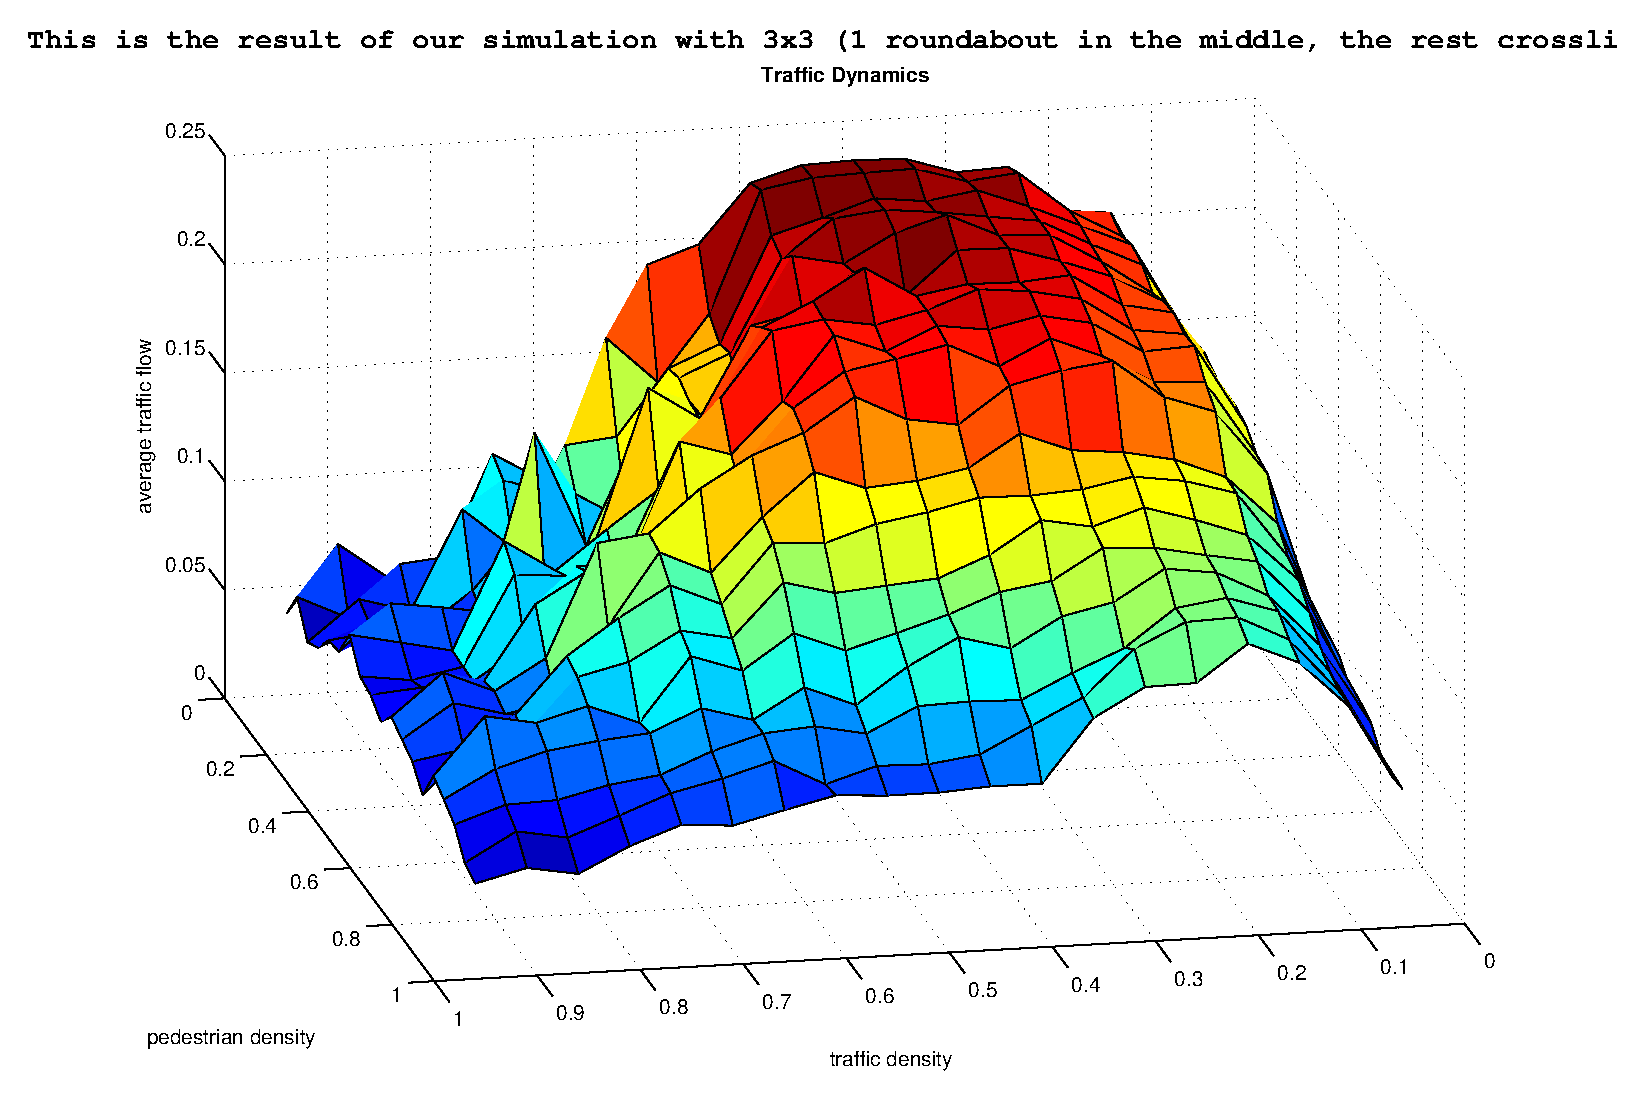
\includegraphics[width=15cm]{images/3-3-mix.eps}

Here it is visible, that just one roundabout in the middle is able to block for high pedestrian densities, were as for lower ones this is clearly dominated by the eight trafficlights. \\

Here we also want to mention that we wrote our programm in a way to run our simulations on more than one computer. To simulate we used 4 student computers from ETH which were running for 2h in parallel to produce the results shown above.


